\chapter{Two-dimensional Grain Growth}
\label{chap:2dgrains}

\lettrine{G}{rain} growth in polycristalline materials is studied over thin film that is a simplification of real three-dimensional grain structures. 
This structure is composed by grains and boundaries. 
Each boundary is shared by two grains and the point where three junctions (and also three grains) meet is called a vertex or triple junction. 
General topology also admits more than three neighbor vertices, however we will only take into account in the models the existence of triple junctions, naming them indistinctly as vertices as well.
Formally, the mathematical description of a grain structure is defined over the unit squared domain $\dom$ with periodic boundary conditions, thus the domain is a torus. 
The grain structure is composed by a disjoint set of $N$ regions over the whole domain. 
We denote this set as,
\begin{equation}
    \grains = \grains(t) = \left \{ \grn^{(1)}, \grn^{(2)}, \dotsc, \grn^{(N)} \right \},\quad N=N(t).
    \label{eq:grainsdef}
\end{equation}
Note that the number of grains varies over time, which is indicated in the temporal dependence notation. 
With each grain $\grn^{(l)},\; l = 1,\dotsc, N$ we associate an orientation $\alpha_l \in [0, 2\pi)$. 
The grains are limited by their boundaries. 
The boundary set is defined as,
\begin{equation}
    \boundaries = \boundaries(t) = \{\bnd^{(1)}, \bnd^{(2)}, \dotsc, \bnd^{(K)}\},\quad K=K(t).
    \label{eq:boundariesdef}
\end{equation}
Again, the number of boundaries in the system also depends on time. 
The grain misorientation parameter $\Delta \alpha^{(k)}$ is defined as$\Delta \alpha^{(k)} = \alpha_{l_2} - \alpha_{l_1},\;k = 1,\dotsc,K$ where $l_1$ and $l_2$ are the indices of the two grains adjacent to the $k$-th boundary. The grain boundary energy $\gamma^{(k)}$ is assumed to depend only on the grain misorientation parameter, 
that is $\gamma^{(k)} = \gamma(\Delta \alpha^{(k)}),\; k = 1,\dotsc,K$ and some even periodic function $\gamma: \Reals \rightarrow \Reals$. 
In this work we will use the grain energy function defined in~\cite{Kinderlehrer2006} which is,
\begin{equation}
    \gamma^{(k)}(\Delta \alpha) = 1 + \frac{\varepsilon}{2}\left(1-\cos^3(4\Delta\alpha)\right)
    \label{eq:gamma}.
\end{equation}
If we set $\varepsilon = 0$ all the energies will be equal to 1, which we call \emph{isotropic setting}. 
Other values of $\varepsilon$ yields the \emph{anisotropic setting}, giving different values of energy for each boundary.
%
Each boundary is parametrized as a curve in the plane defined as:
\begin{equation}
    \bnd^{(k)}(t) = \left\{ \vxi^{(k)}(s,t), \quad s \in [0, 1] \right\},\quad k = 1, \dotsc, K.
    \label{eq:grainboundary}
\end{equation}
As stated previously, boundaries meet at triple junctions, and these correspond to the start or the end point of exactly three boundaries. 
We denote the set of triple junctions as,
\begin{equation}
    \vertices = \vertices(t) = \left\{ \x_1, \x_2, \dotsc, \x_M \right\},\quad M = M(t).
\end{equation}
Let $\bnd^{(k_1)}, \bnd^{(k_2)}, \bnd^{(k_3)}$ three different boundaries with a common triple junction $\x_m$. For the curve parameters $s_{k_i} = \{0,1\}$ the triple junctions are defined in function of the boundaries as
\begin{equation*}
    \x_{m}(t) =  \vxi^{(k_1)} (s_{k_1},t) = \vxi^{(k_2)} (s_{k_2},t) = \vxi^{(k_3)} (s_{k_3},t),\quad m =1,\dotsc,M.
\end{equation*}
%
Figure~\ref{fig:grainstructure} shows a simulated grain structures under the given definition.
% \begin{figure}[t]
%     \centering
%     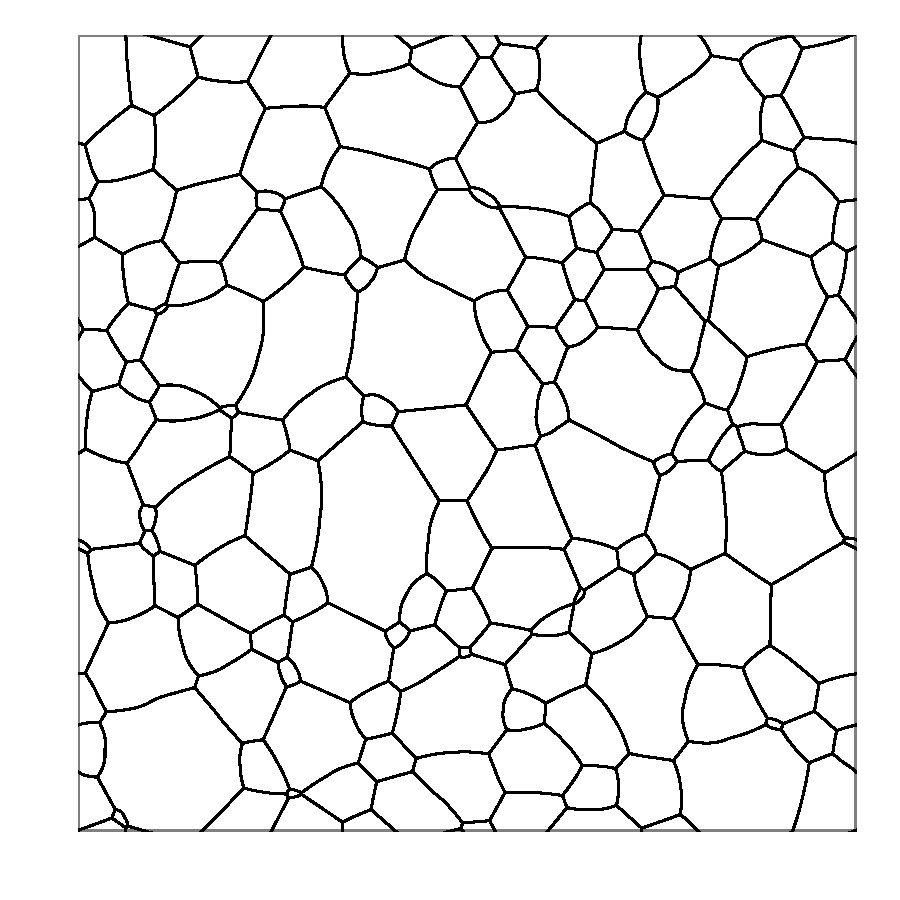
\includegraphics[scale=0.5]{twodim/grainstructure.pdf}
%     \caption{Simulated grain structure under periodic boundary conditions.}
%     \label{fig:grainstructure}
% \end{figure}
\begin{figure}[t]
    \centering
    \subfloat[Vertex-based structure]{
    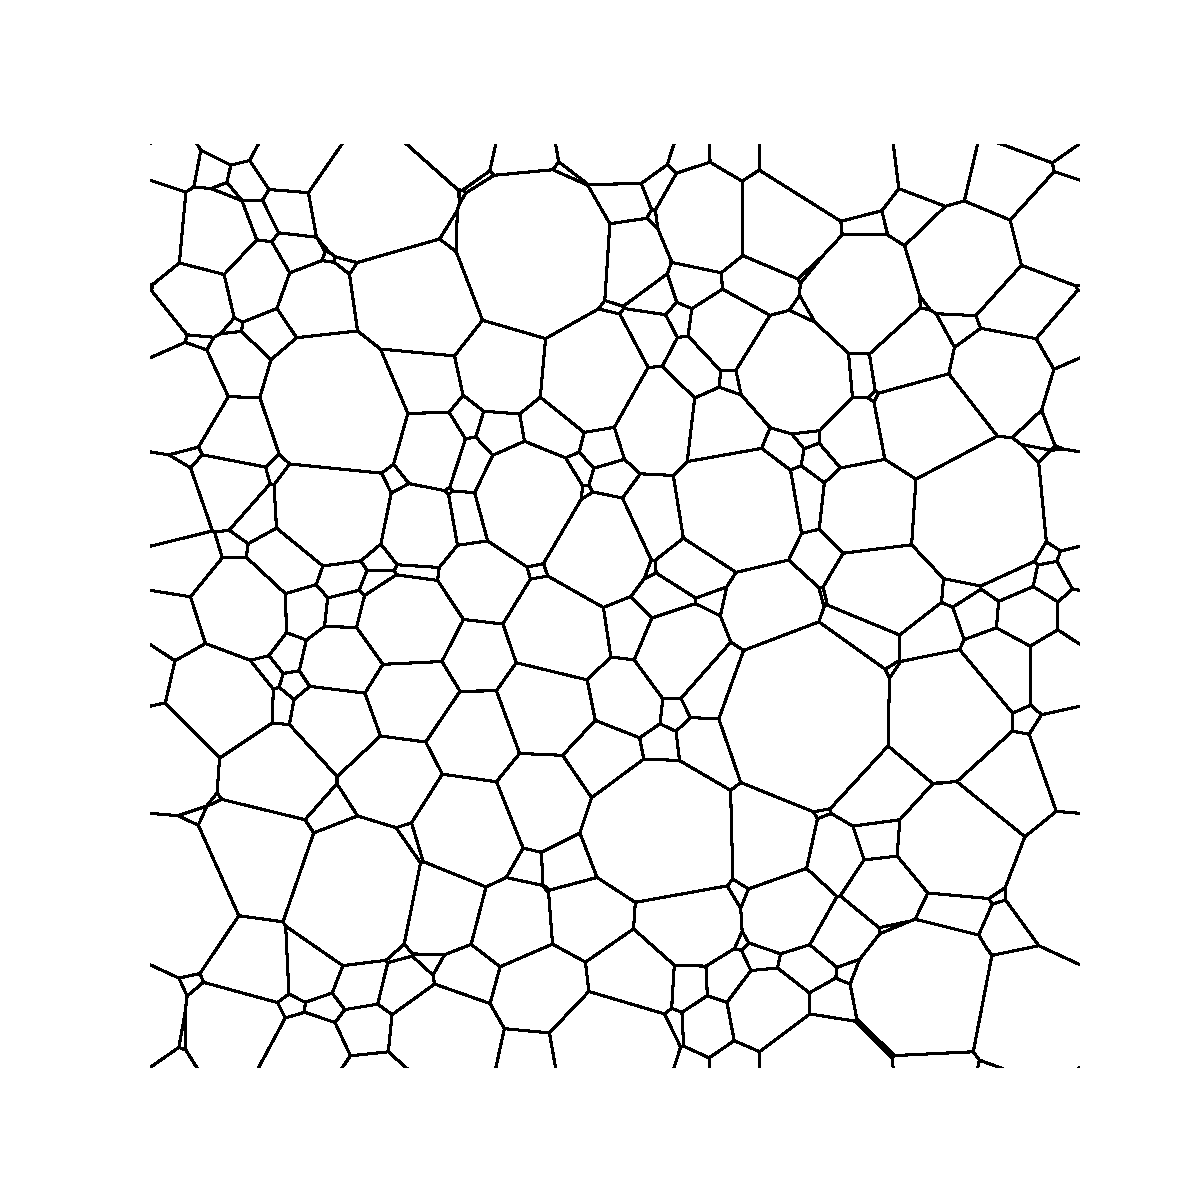
\includegraphics[scale=0.37, trim={2em 2em 2em 2em}]{figures/twodim/gs_vertex.pdf}
    }%
    \subfloat[Curvature-based structure]{
    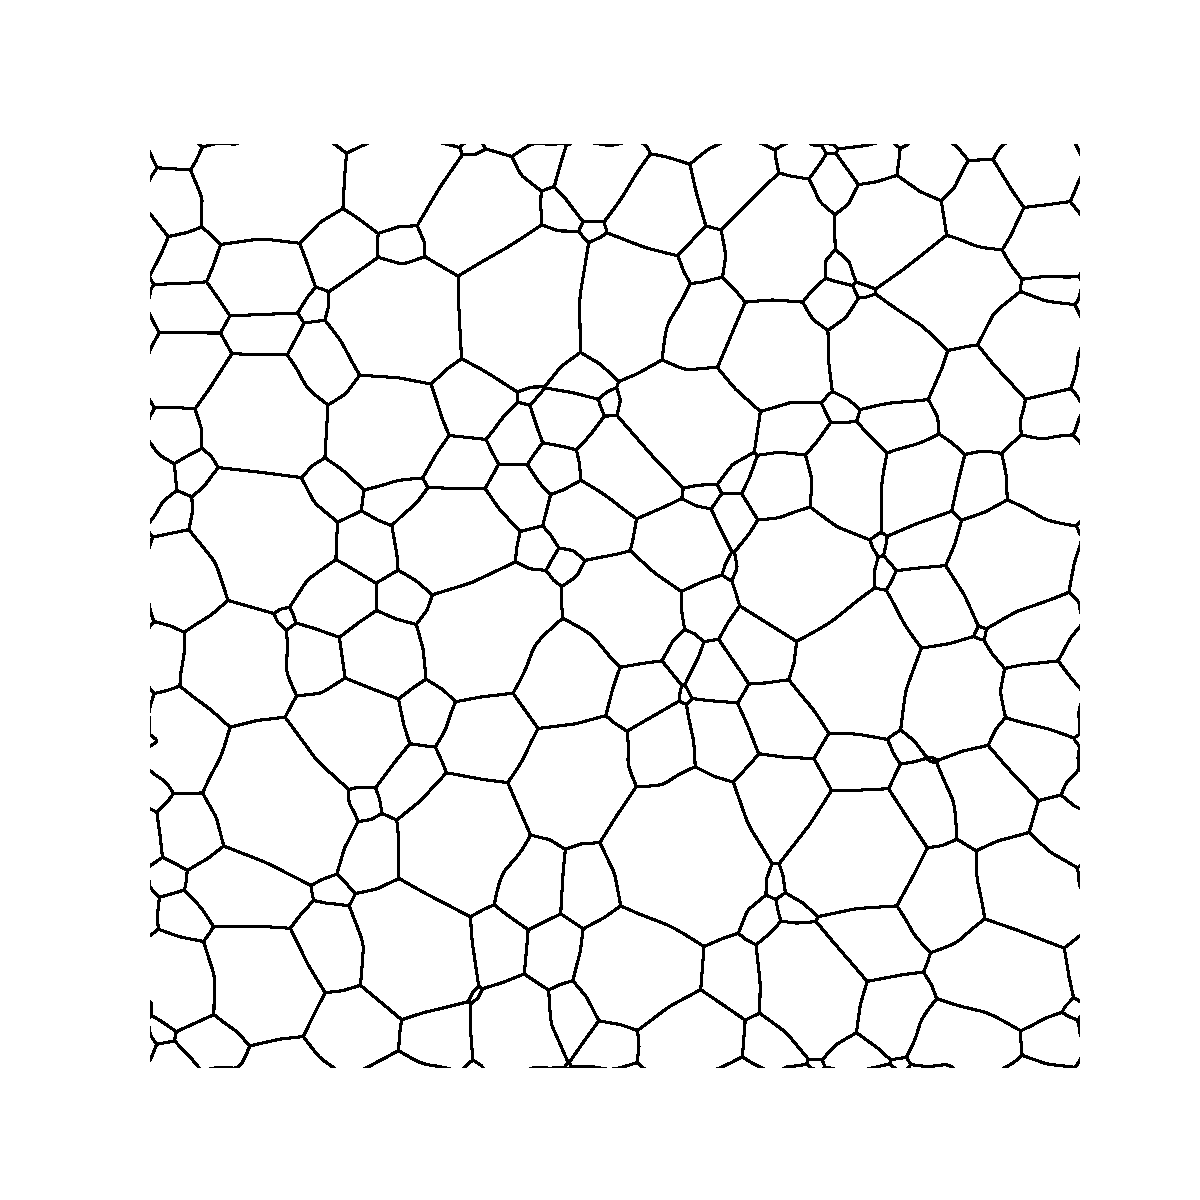
\includegraphics[scale=0.37, trim={2em 2em 2em 2em}]{figures/twodim/gs_curvature.pdf}
    }
    \caption{Simulated grain structures under periodic boundary conditions.}
    \label{fig:grainstructure}
\end{figure}
As discussed before, the grain system evolves over time, vertices and boundaries moves, some grains shrink and other grow. 
When a boundary decreases its length to zero, or when a grain area becomes zero, a component of the system disappears. 
These changes are denominated topological transitions and are described in the next section, see Section \ref{sec:topological_transitions}.

\section{Topological Transitions}\label{sec:topological_transitions}

Topological transitions are the result of coarsening during grain growth and are well documented by Ferro et al.~\cite{ferro1997elimination}. 
%They dependent on the grain boundary energy $\gamma$, thus some configurations are more probable than others. 
The most common handled topological transitions~\cite{kinderlehrermultiscale, Kinderlehrer2006, torres2015, van2016curvature} in grain growth models are neighbor switching (also known as flipping) and grain removal, as shown in Figures~\ref{fig:flipping} and~\ref{fig:removal}.
The addition of a new grain into the system, also called nucleation, it is a type of topological transition that happens in primary recrystallization before grain growth. Along with this transition, other types of transition related to nucleation have
been documented, but they will not be included here, see~\cite{pikekos2008stochastic}.

\begin{figure}[t]
    \centering
    \subfloat[Neighbor flipping.]{
        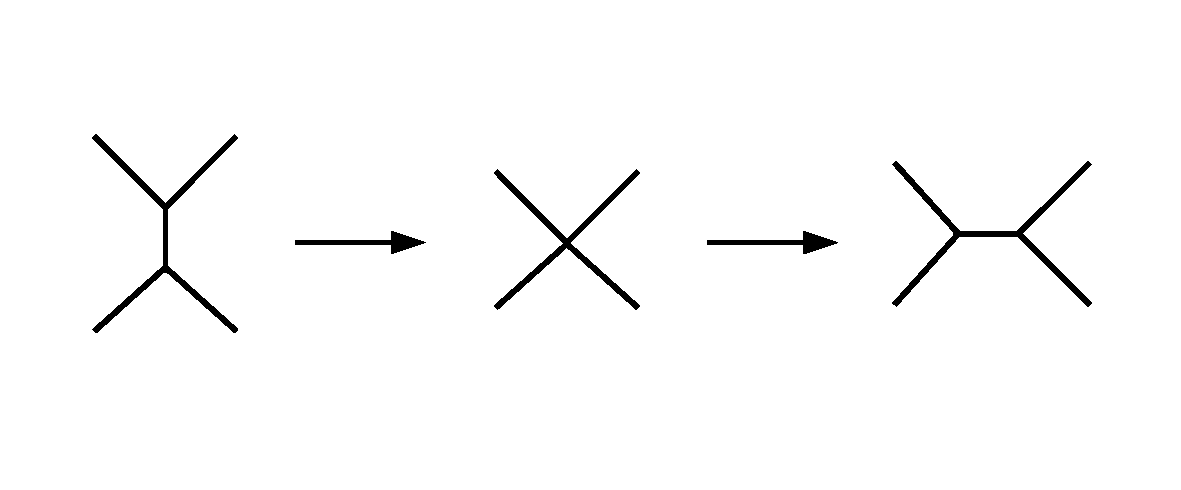
\includegraphics[scale=0.5]{twodim/flipping.pdf}
        \label{fig:flipping}
    }\\
    \subfloat[Grain removal.]{
        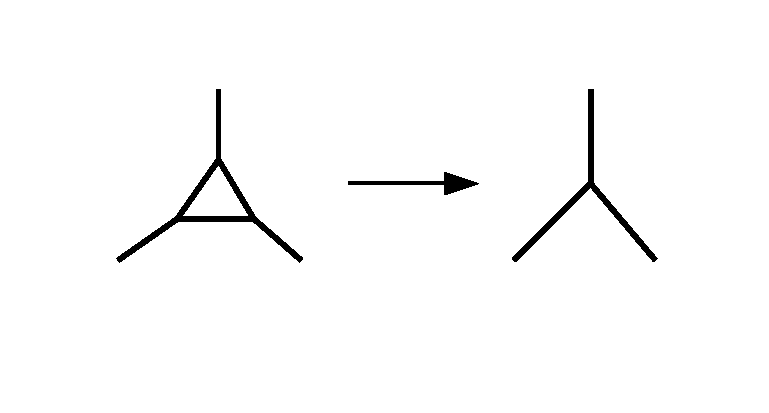
\includegraphics[scale=0.5]{twodim/removal.pdf}
        \label{fig:removal}
    }%
    \subfloat[Nucleation in a vertex.]{
        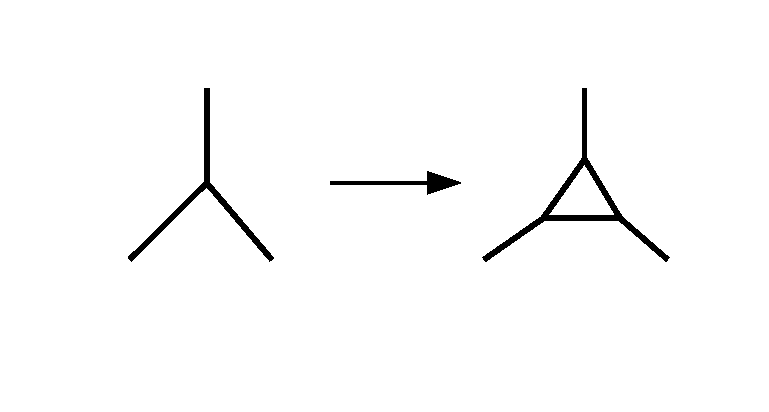
\includegraphics[scale=0.5]{twodim/nucleation.pdf}
        \label{fig:nucleation}
    }
\end{figure}

Neighbor flipping (Figure~\ref{fig:flipping}) consist in a grain boundary switching neighboring boundaries. 
This occurs when a boundary collapses, the vertices approach each other, decreasing the boundary length to zero. 
This configuration, called a quadruple junction since it involves four boundaries, is unstable under the regimes studied and breaks in two new vertices and the new boundary grows in a new direction.

Grain removal (Figure~\ref{fig:removal}) consists in the removal of a grain which decreased its area to zero. 
The grain then is replaced by a group of boundaries or a single vertex. In~\cite{ferro1997elimination} are shown different configurations of grains and how they are arranged after grain removals. We focus only in the removal of three sided grains.
%There are many results from grain removal that arise from different configurations, but the most important is the disappearing of a three-sided grain. 
A three sided grain is removed when one or more of its boundaries switch neighbors. 
This will generate a degenerated grain with two sides. Instead of that, a new vertex is created and the boundaries adjacent to the former grain are now joined. 

It is possible that a grain being removed takes part of a configuration where one of its neighbors also has three sides. 
In this case the grain removal generates another two-sided grain that is not valid in the network and for network consistency we can either stop the simulation or repair completely the structure by replacing the two three-sided grains by a single boundary.

Nucleation (Figure~\ref{fig:nucleation}) consists in the addition of a grain in the grain system. The energetic conditions and the site in the grain structure to add the new grain (on a boundary, vertex or inside another grain) are part of the primary recrystallization phenomenon (see~\cite{pikekos2008stochastic, pikekos2008generalized, Piekos2004}). Chapter~\ref{chap:storedenergy} addresses a Vertex Model that is able to produce this transition.



\section{Topology of Grain Structures}

As stated before, the grain structure is projected on a torus where each vertex is connected to three other vertices, and thus belongs to three boundaries. 
The structure has the following Euler characteristic considering the number of vertices $M$, the number of boundaries $K$ and the number of grains $N$~\cite{sausset2007periodic}:
\begin{equation}
M - K + N = 0.
\label{eq:eulertorus}
\end{equation}
If we count the number of vertices in a grain structure we count three boundaries per vertex, but as each boundary is shared by two vertices, the boundaries are counted twice. Using these facts and considering \eqref{eq:eulertorus} we obtain the following relations:
\begin{align*}
    3\,M &= 2\,K & 
    N &= \frac{K}{3} = \frac{M}{2}.
\end{align*}
Consider an initial condition of a grain structure with $N_0$ number of grains, $M_0$ vertices and $K_0$ boundaries where $N_0 = M_0/2 = K_0 / 3$. 
The topological transitions during grain structure evolution will change the number of these components. 
The only topological transition considered that alter the number of components in a grain structure is  grain removal.
When a grain is removed, three boundaries and two vertices are removed, leaving a single \emph{survivor} vertex.
Now assume that at a given time $t$ we started with $N_t$ grains and then we removed $n_t$ grains, leaving at the next time step $N_{t+1}$ grains, $N_{t+1} < N_{t}$. 
Topological transitions described induces that we removed exactly $3\,n_t$ boundaries and $2\,n_t$ vertices and the following definitions yields between vertices, boundaries and grains between time steps $t$ and $t+1$:
 \begin{align*}
     dN_t &= N_{t+1} - N_{t} =  - n_t\\
     dK_t &= K_{t+1} - K_{t} = - 3n_t\\
     dM_t &= M_{t+1} - M_{t} = - 2n_t.
 \end{align*}
We can build the following relation in terms of the variation of grains as
\begin{equation}
    3\,dM_t = 2\,dK_t. \label{eq:dMdK}
\end{equation}
If we add the variations over all the time steps, from time $t=0$ to $t=T$ we obtain
\begin{align*}
    \sum_{t=0}^{T}3\,dM_t &= 3(M_1 - M_0 + M_2 - M_1 + \cdots + M_{T+1} - M_T) \\
    &= 3(M_{T+1} - M_0).
\end{align*}
\begin{align*}
    \sum_{t=0}^{T}2\,dK_t &= 2(K_1 - K_0 + K_2 - K_1 + \cdots + K_{T+1} - K_T) \\
    &= 2(K_{T+1} - K_0).
\end{align*}
This total variations for vertices and boundaries are equal according to \eqref{eq:dMdK}. 
Under the fact that the initial condition is true, \ie  $3M_0 = 2K_0$, for a time $t=T$ the number of vertices and boundaries are related as,
\begin{align*}
    N_{T+1} &= \frac{M_{T+1}}{2},
    & N_{T+1} &= \frac{K_{T+1}}{3},
    & 3\,M_{T+1} &= 2\,K_{T+1}.
\end{align*}
This implies that grain structure evolution holds the same relation between grains, boundaries and vertices along the simulation.

%%% Dynamics
\section{Curvature and Vertex Models}
%
The total energy of the grain structure depends on the individual energies along each grain boundary. 
The total energy thus takes the form,
\begin{equation}
    E(t) = \sum_{k=1}^{K} \int_0^1 \gamma ^{(k)}\norm{\mylvec^{(k)}(s,t)}\, ds,
    \label{eq:energy}
\end{equation}
where $\mylvec^{(k)}(s,t) = \dxids^{(k)}(s,t)$ is a tangent vector to $\vxi^{(k)}$ and $\norm{\cdot}$ is the $l^2$-norm. Grain network evolution equations can be found from this equation by taking the derivative of the energy with respect to time. 
Computing the derivative of $\eqref{eq:energy}$ we obtain,
\begin{align}
    \dfrac{dE}{dt}(t) &= \sum_{k=1}^{K} \int_0^1 \gamma^{(k)} \unitlk \cdot \dlvecdt^{(k)}\!(s,t) \, ds \nonumber\\
    &= \sum_{k=1}^{K} \int_0^1 \gamma^{(k)}\, \T^{(k)}(s,t) \cdot \dvds^{(k)}\!(s,t) \, ds \label{eq:dEdt},
\end{align}
where $\T^{(k)}(s,t)$ is a unit tangent vector of the boundary and $\gamma^{(k)}\T^{(k)}$ it is called capillar force. 
Note that \eqref{eq:dEdt} is valid as long as $K'(t) = 0$ within $[t_1, t_2]$, \ie
there are not topological transitions. 
Integrating by parts \eqref{eq:dEdt} we obtain,
\begin{equation}
    \dfrac{dE}{dt}(t) = -\sum_{k=1}^K \int_0^1 \gamma^{(k)}\dTds^{(k)}\!\!\cdot \vel^{(k)}\, ds + \sum_{m=1}^M \vel_m \cdot \sum_{l=1}^{3} \gamma^{(m,l)}\T^{(m,l)}
    \label{eq:dEdtfull},
\end{equation}
In order to enforce the decreasing energy of the system we must ensure that \eqref{eq:dEdtfull} be negative. 
If we only consider the triple junction drag the boundaries becomes flat, therefore $\dTds^{(k)}\! = 0$ for each boundary. 
The triple junction velocity is set to decrease energy as,
\begin{equation*}
    \vel_{m} = - \lambda \gamma^{(m,l)}\T^{(m,l)},
\end{equation*}
where $\lambda$ is called triple junction mobility. 
This model is called \emph{Vertex model}. 

On the other hand if we only consider the grain boundary influence, we can set the velocity to be proportional to the boundary normal vector, which yields the following expression for boundary velocity:
\begin{equation*}
    \vel^{(k)} = \mu \gamma^{(k)} \dTds^{(k)},
\end{equation*}
where $\mu$ is called boundary mobility. 
Since the motion is curvature-driven,\ie there is no triple junction influence, this model is called \emph{Curvature model}. 
A geometrical consequence under this model is the \emph{Herring condition} where the angle between boundaries, namely dihedral angle, is always $2\pi/3$~\cite{herring1951surface}. 
This comes from forcing the geometrical condition over tangent vectors:
\begin{equation}
    \sum_{l=1}^{3}\gamma^{(m,l)}\T^{(m,l)} = 0.
\end{equation}
Moreover the rate of growth for a grain becomes independent of its area, 
being proportional to the number of sides of the grain or grain class $\ns(\grn)$. 
This relation establishes that a grain with $\ns(\grn) < 6$ will shrink and with $\ns(\grn) > 6$ will grow, in fact the case of 6-sided grain the rate of growth is zero. 
This relation is known as \emph{Von Neumann-Mullins relation}~\cite{mullins1956two} and can be expressed as
\begin{equation}
    \frac{dA}{dt}(\grn) = \frac{\nu}{3}(\ns(\grn)-6)
    \label{eq:vonneumann-mullins}
\end{equation}
where $\nu$ is a term proportional to grain boundary energies $\gamma^{(k)}$ and mobility $\mu$. 
%Under constant $\gamma^{(k)}$, $\nu \propto \gamma \mu$.
